%%%%%%%%%%%%%%%%%%%%%%%%%%%%%%%%%%%%%%%%%%%%%%%%%%%%%%%%%%%%%%%%%%%%%%%%%%%
% 1) INTRO
%%%%%%%%%%%%%%%%%%%%%%%%%%%%%%%%%%%%%%%%%%%%%%%%%%%%%%%%%%%%%%%%%%%%%%%%%%%

\section{Introduction}
\label{s:intro}

%Making a conscious effort to remove "britishisms" from the text -- thus, hence, whilst, while, yet, whereas, etc. 
%Also trying to slim down on adjectives. One mans's "very" is another man's "some". 
%To make diff/merge easier. I am now putting 1 "statement" (sentence) per line. 
%Trying to apply the KISS principle, especially to the language used, to help out our American reviewers. 

By classical wisdom, smaller packet headers are better: fewer bits wasted on the wire mean greater efficiency overall. 
Van Jacobson's impressive RFC~1144~\cite{rfc1144} ``\emph{Compressing TCP/IP Headers for Low-Speed Serial Links}'' takes this concept to the extreme.
It shows how to compress the 40 byte TCP/IP header down to less than 4 bytes in the common case. 


Despite the heroic efforts of Jacobson and others to keep TCP/IP headers short, saving bits on the wire is only beneficial if the cost of transmission outweighs the cost of compression. 
For example, on a 9600b/s serial link, each bit costs around 10 microseconds to transmit. 
By saving 36 bytes per packet, Jacobson could save just under 30 milliseconds per transmission.
From a total round trip budget of 100 milliseconds, 30 milliseconds represented an impressive saving.


On a modern 40Gb/s Ethernet link, each bit now costs 25 picoseconds to transmit.
A best-in-class CPU running at 4GHz executes only one cycle every 250 picoseconds. 
This means that the CPU needs to be able to process an average of 10 bits per cycle to keep up with line-rate. 
As we go forward, power and thermal efficiency issues are causing CPUs to get slower and wider rather than faster. 
Intel's new Haswell CPUs typically execute 1 cycle every 500 picoseconds (2GHz). 
By contrast, networks are getting faster. A 100Gb/s Ethernet link can transmit 1 bit every 10 picoseconds, a factor of 50x faster. 
This means that CPUs now need to process on average 50 bits per cycle just to keep up. 
%This leaves no time for handling anything other than packet processing. 


A 64-bit CPU should be able to cope with 64 bits per cycle, as long as each instruction requires only one cycle. % and it operates on the whole 64 bits at once.
Modern CPUs typically require multiple cycles for many instructions.
By packing bits tightly together and by aligning fields on 16-bit (Ethernet) or 32-bit (TCP/IP) boundaries, we guarantee that the CPU will need to do more than 1 instruction per header field. 


\begin{figure}
 \centering
 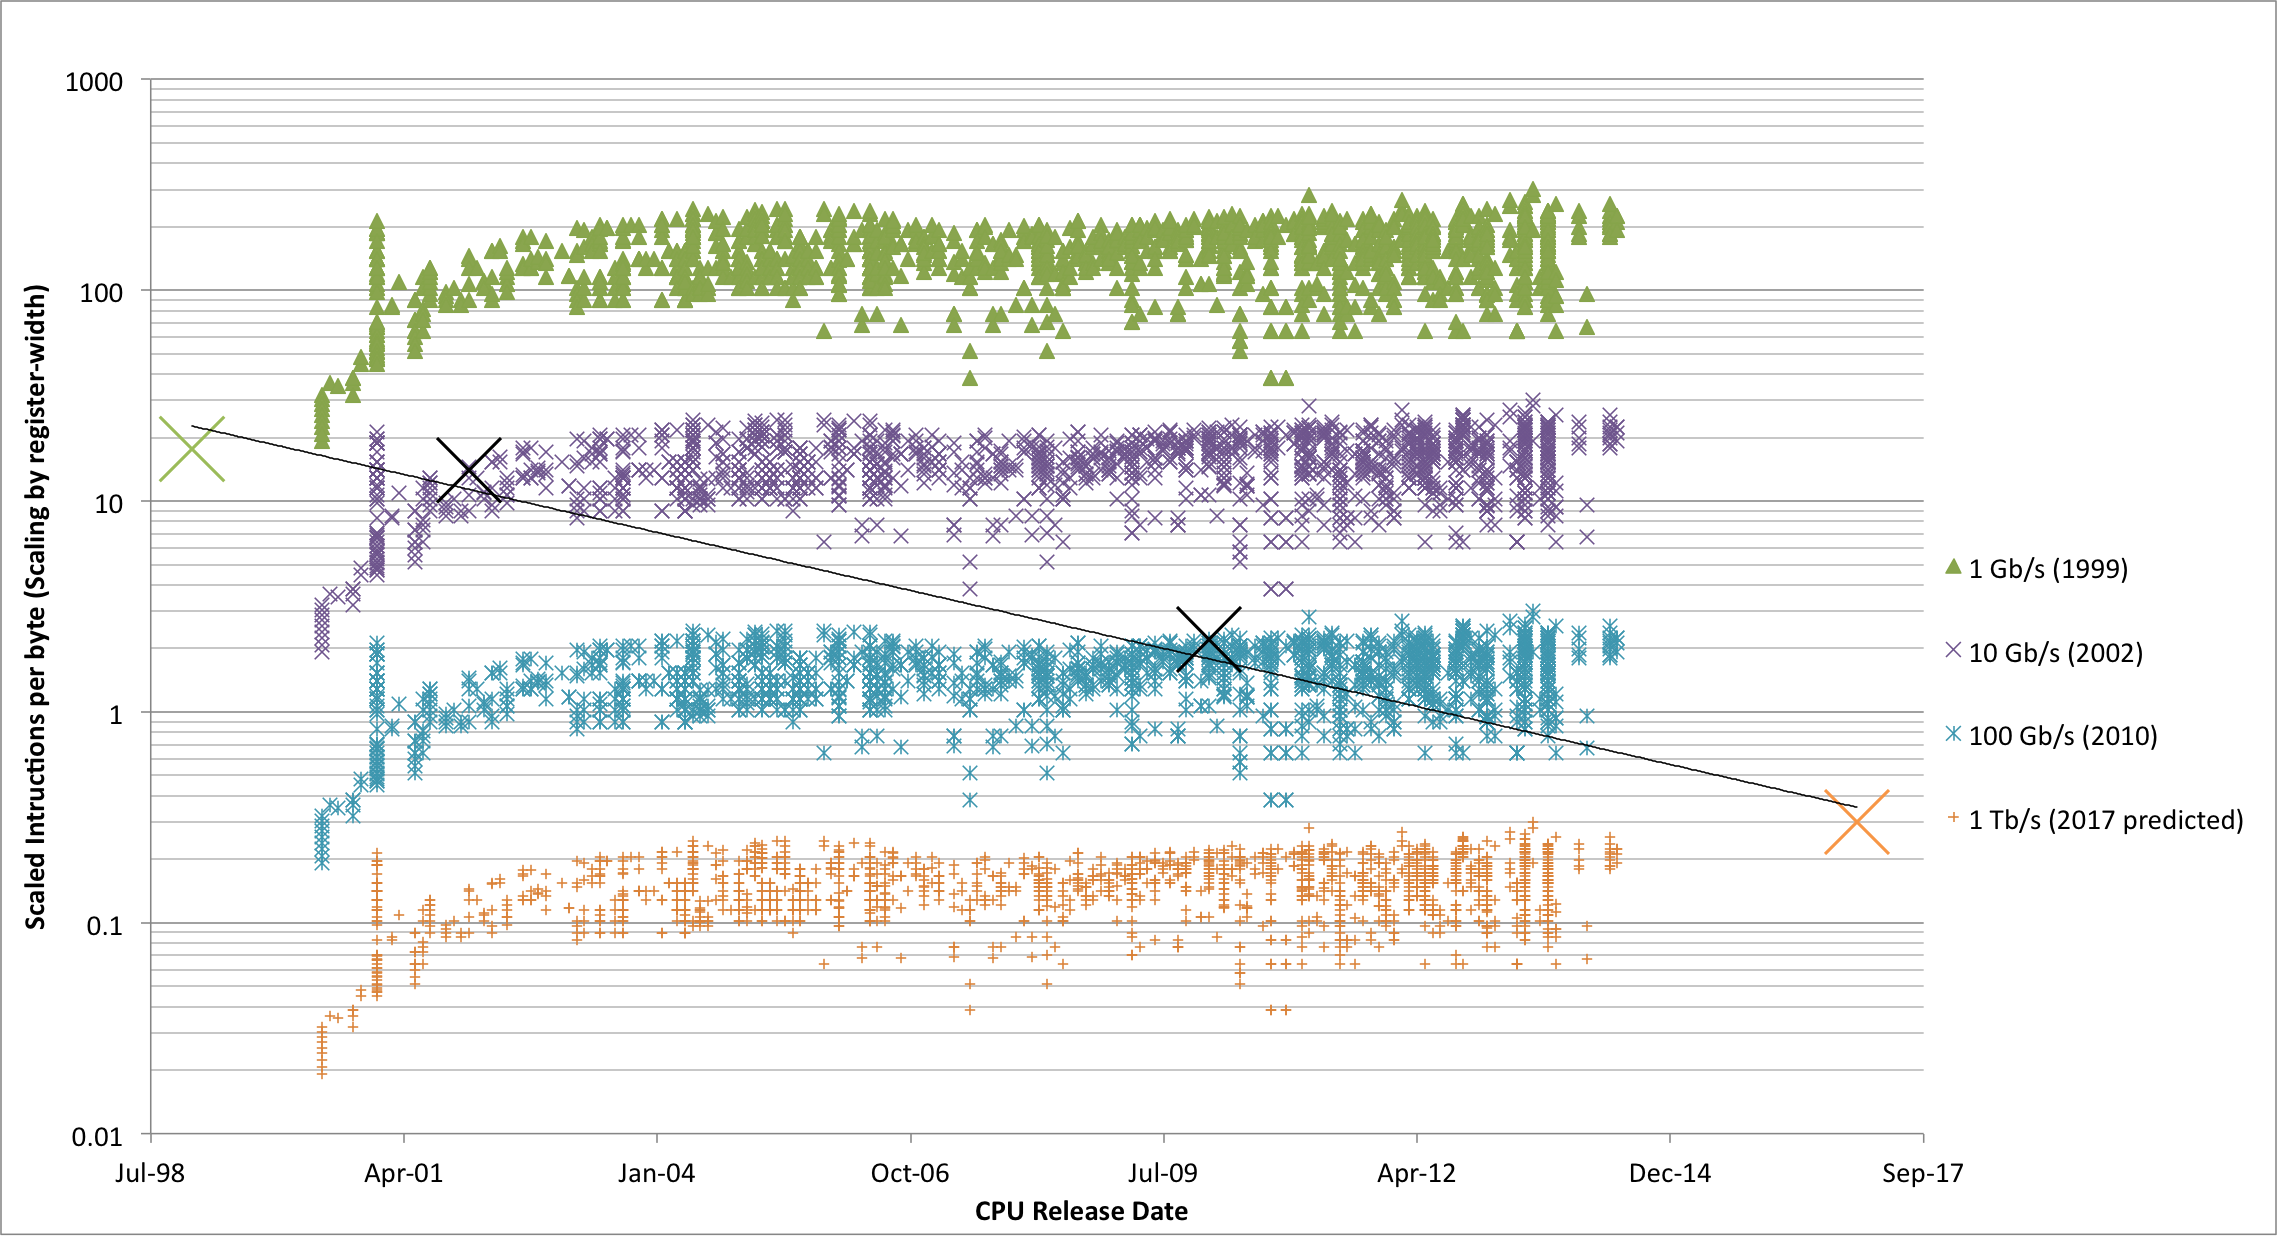
\includegraphics[width=1\columnwidth]{figures/cpu/ips-figure.png}
 \caption{Instructions per network-byte for a range of Ethernet technologies. Despite scaling by instruction width, the flattening of CPU instruction-rate is clear.  }
 \label{f:ips-figure}
\end{figure}



It gets worse. 
Network packets are transmitted using network byte ordering which is "big-endian", but the majority of CPUs today use "little-endian" byte ordering internally. 
Once the CPU has found and extracted the correct field from a packet, it then needs to reorder the bytes into little-endian format. % before it can do anything useful with them. 
The little-endian conversion adds strain to an already tight cycle budget.


From these examples, it should be clear that CPU cycles are becoming a rare commodity and that network bits are now plentiful. We think that the time has come to reevaluate the tradeoffs in on-the-wire formats for TCP/IP protocols. 
Specifically, we consider if there are optimisations to the layout of packets in host memory only, without changing the functionality of the protocols themselves. 
To do this, we build a simple network stack that runs directly out of host memory. 
We then test a variety of different packet layouts and show that gains of nearly 3$\times{}$ can be found by arranging packet wire formats correctly, allowing network stacks to scale beyond 40Gb/s and up to over 100Gb/s. 


%Ultimately we show how to build a simple network stack, capable of processing above 100Gb/s on a single core. 
%By applying optimisations to this stack, we can test the limits of CPU based network processing. Since our stack in minimal and our CPU is fast, our experiments represent the absolute limit. Our "application" emulation simply reads intergers out of the packet in an array and in


%For an intuitive sense of the problem, consider a 

%
%We consider the following questions: 
%- Can expanding the number of bits assigned to a given field reduce the overall processing time, despite a modest increase in the transmission time. 
%- Is the big endian “network” byte order costing more than it benefits considering that the majority of machines in operation are little endian.
%- Is it necessary that packet layout reflects layering found in the protocol stack, or are there optimisations to be found by rearranging packet contents. 
%- Can these optimisations be made transparently to the network legacy network stack in much the same way that Van Jacobson achieved header compression. 
%
%Evaluation Proposal: 
%- Instrument linux (and? BSD) stack - Count the cycles it takes to process UDP/TCP/ICMP/ARP - Count the min/max/med/ave/std-dev cycles per bit. 
%- Build a simple UDP/ICMP/ARP (maybe using Netmap or DPDK) that is faster than Linux. 
%- Since our stack is faster than linux, it must necessarily be doing less work per bit. Count the min/max/med/ave/std-dev cycles per bit. 
%- Show that we can do even less work (cycles and/or instructions) by expanding the headers. Compare the Count the min/max/med/ave/std-dev cycles per bit. to above. 
%
%(Maybe do this for both ipv4 and ipv6) 
%
%Conclude that we can make cycles per bit go down by expanding headers, and predict what this will mean for near future cpu architectures/very high link speeds. 
